\documentclass[../../main.tex]{subfiles}
 
\begin{document}

\begin{table}
\small
\centering
\begin{tabular}{| c | c | c | c | c | c | c |}
\hline \hline
Question & 135A $N$ & 135A Mean & 135A Std. dev. & 135B $N$ & 135B Mean & 135B Std. dev. \\ \hline
10 & 21 & 3.76 & 1.04 & 18 & 3.72 & 0.96 \\ \hline
11 & 21 & 4.57 & 0.75 & 18 & 4.78 & 0.43 \\ \hline
12 & 21 & 4.29 & 1.01 & 18 & 3.78 & 1.00 \\ \hline
13 & 21 & 3.52 & 1.33 & 18 & 3.33 & 1.53 \\ \hline
14 & 21 & 3.48 & 1.36 & 18 & 2.72 & 1.32 \\ \hline
15 & 21 & 3.29 & 1.68 & 18 & 2.28 & 1.53 \\ \hline
16 & 21 & 3.19 & 1.57 & 18 & 2.94 & 1.30 \\ \hline
\hline
\end{tabular}
\caption{\label{tab:courses:intro_eval_1} Summary of questions 10-16 on the student evaluation form, for PHYS135A/B taught in Fall 2017 and Spring 2018.  These questions pertain to the \textit{course}.}
\end{table}

\begin{table}
\centering
\begin{tabular}{| c | c | c | c | c | c | c |}
\hline \hline
Question & 135A $N$ & 135A Mean & 135A Std. dev. & 135B $N$ & 135B Mean & 135B Std. dev. \\ \hline
17 & 21 & 4.24 & 1.04 & 18 & 3.67 & 1.03 \\ \hline
18 & 21 & 3.52 & 1.33 & 18 & 3.11 & 1.57 \\ \hline
19 & 21 & 3.48 & 1.40 & 18 & 2.89 & 1.29 \\ \hline
20 & 21 & 4.24 & 1.09 & 18 & 4.06 & 1.25 \\ \hline
21 & 21 & 4.48 & 1.03 & 18 & 3.78 & 1.17 \\ \hline
22 & 21 & 4.10 & 0.89 & 18 & 3.88 & 1.02 \\ \hline
23 & 21 & 3.95 & 1.20 & 18 & 3.53 & 1.33 \\ \hline
24 & 21 & 4.67 & 0.58 & 18 & 4.24 & 0.97 \\ \hline
25 & 21 & 3.24 & 1.55 & 18 & 3.12 & 1.36 \\ \hline
\hline
\end{tabular}
\caption{\label{tab:courses:intro_eval_2} Summary of questions 17-25 on the student evaluation form, for PHYS135A/B taught in Fall 2017 and Spring 2018.  These questions pertain to the \textit{professor}.}
\end{table}

Tables \ref{tab:courses:intro_eval_1} and \ref{tab:courses:intro_eval_2} show the results of the \textit{algebra-based} introductory physics courses taught in the 2017-2018 academic year.  Tables \ref{tab:courses:intro_eval_3} and \ref{tab:courses:intro_eval_4} show the results of the \textit{calculus-based} introductory physics courses taught in the 2017-2018 academic year.  The results show an interesting correlation that reveals a potential strategy for continual improvement of my teaching in these courses. \\ \hspace{0.1cm}

First, there are obvious areas that need improvement.  Questions 14-16 and 19 for 135B for example correspond to student understanding of the material, interest in the material, recommending the course to others, and my ability to explain complicated ideas, respectively.  This particular algebra-based course is meant to cover electricity and magnetism.  We introduce students without a technical background to abstract ideas like electromagnetic fields and how they connect to applications like DC circuits.  Skills necessary to complete the work in this course include solving algebraic equations and systems of equations, analyzing graphs of functions, and correctly measuring properties of circuits and magnets.  It is no surprise that students struggle with the material upon encountering it for the first time.  I have been trained to teach much faster and more intensely than the students who disapproved of the course desired. \\ \hspace{0.1cm}

On the other hand, there are many areas in which the courses and my teaching scored well.  Students in both sections believed that the courses were rigorous and challenging.  Some students appreciated the PI modules, PhET simulations, and JITT exercises.  This is reflected in responses to question 12 on the standard evaluation, which is a key data point.  The reason I focus on this data point is that I am being asked by my department to teach in an activities based style, far different from the traditional lecture format.  The purpose of the activities and group exercises is to satisfy the focus on \textbf{improvement of analysis skill}.  The PI, JITT, and PhET modules are constructed to improve analysis skill.  However, upon reflecting on the students' constructive comments, it seems that these modules benefit some students but not all. \\ \hspace{0.1cm}

In the students' remarks, many shared with me that these courses were the very first physics courses they have taken, or that they have anxieties with mathematics.  In consultation with my department chair, and in studying past PEGP documents in my department, it appears that an increase in traditional lecture style is necessary.  The reason is that if every single concept and number in physics is confusing to a first-time student, then merely updating the teaching style with researched-based modules will not help that student.  The traditional lecture style offers the benefit that students see many example problems done in explicit detail, such that they can copy and repeat the technique.  I was taught to never expect this as an undergraduate student, because it is wrong.  My colleagues in my department have reassured me that it is not only not wrong, but necessary to give inexperienced students an explicit starting point.  Thus, this will be the first major change to my introductory teaching this coming semester: \textit{fifty percent of class-time will be spent on concrete examples in the traditional style.} \\ \hspace{0.1cm}

The second major change I will be making to my introductory course teaching style is to slow the pace.  In reading students' remarks, this is the second most common desire on their part.  I was taught at the undergraduate and graduate levels at high speed, with intense focus on both content and mathematical detail.  Of course I must make adjustments for the environment at Whittier College, and not merely teach to myself.  I must \textit{teach to the middle}, as one of my colleagues recommended.  The students felt major relief when I began assigning them a problem to work on the whiteboards in groups precisely because it allowed them to slow the class down, and check their work with each other.  Thus, that move solved both problems at once: the problem of pace and the problem of adding more traditional lecture content.  The students got a chance to lecture to each other momentarily.  In the upcoming semester, \textit{I will include the group-board technique in the normal course plan}. \\ \hspace{0.1cm}

Third, I'd like to include calculus in the \textit{calculus-based} versions of our introductory sequences.  Currently, our department does not include enough calculus-based content in PHYS150 and PHYS180.  However, I am congizant of the risks in adding content to these courses, in which we are already pushing the majority of students to their limits.  From the feedback from my department, I need to include more laboratory/measurement activities.  Thus, I propose solving both problems simultaneously.  When I teach \textit{calculus-based} introductory courses in the future, I will use the laboratory activities as a venue for demonstrating the difference between results obtained from calculus (derivatives and integrals) and the average results one obtains without calculus. It is my hope that the students will learn to use some calculus tools, even if the majority cannot deploy calculus in some challenging homework problems.  The inclusion of more lab activities is already required of me, now that I am trained on all of our equipment, so this idea will require no additional effort above what I'm already scheduled to do. \\ \hspace{0.1cm}

\begin{table}
\small
\centering
\begin{tabular}{| c | c | c | c | c | c | c |}
\hline \hline
Question & 150 $N$ & 150 Mean & 150 Std. dev. & 180 $N$ & 180 Mean & 180 Std. dev. \\ \hline
10 & 16 & 4.19 & 0.83 & 18 & 4.00 & 0.91 \\ \hline
11 & 16 & 4.19 & 1.38 & 18 & 4.67 & 0.49 \\ \hline
12 & 16 & 3.63 & 1.31 & 18 & 4.06 & 0.94 \\ \hline
13 & 16 & 4.00 & 1.10 & 18 & 4.00 & 0.97 \\ \hline
14 & 16 & 3.93 & 1.33 & 18 & 3.89 & 0.90 \\ \hline
15 & 16 & 3.56 & 1.26 & 18 & 3.67 & 1.03 \\ \hline
16 & 16 & 3.56 & 1.26 & 18 & 3.83 & 0.86 \\ \hline
\hline
\end{tabular}
\caption{\label{tab:courses:intro_eval_3} Summary of questions 10-16 on the student evaluation form, for PHYS150 taught in Fall 2017, and PHYS1809 taught in Spring 2018.  These questions pertain to the \textit{course}.}
\end{table}

\begin{table}
\centering
\begin{tabular}{| c | c | c | c | c | c | c |}
\hline \hline
Question & 150 $N$ & 150 Mean & 150 Std. dev. & 180 $N$ & 180 Mean & 180 Std. dev. \\ \hline
17 & 16 & 3.31 & 1.14 & 18 & 3.44 & 1.15 \\ \hline
18 & 16 & 2.88 & 1.36 & 18 & 3.39 & 1.14 \\ \hline
19 & 16 & 3.13 & 1.54 & 18 & 3.83 & 1.04 \\ \hline
20 & 16 & 3.69 & 1.25 & 18 & 4.22 & 0.65 \\ \hline
21 & 16 & 3.88 & 1.09 & 18 & 4.11 & 0.96 \\ \hline
22 & 16 & 3.81 & 1.33 & 18 & 4.44 & 0.70 \\ \hline
23 & 16 & 3.67 & 1.37 & 18 & 4.33 & 0.77 \\ \hline
24 & 16 & 4.50 & 0.63 & 18 & 4.56 & 0.51 \\ \hline
25 & 16 & 3.13 & 1.63 & 18 & 3.61 & 1.04 \\ \hline
\hline
\end{tabular}
\caption{\label{tab:courses:intro_eval_4} Summary of questions 17-25 on the student evaluation form, for PHYS150 taught in Fall 2017, and PHYS180 taught in Spring 2018.  These questions pertain to the \textit{professor}.}
\end{table}

Finally, I will put more focus on struggling students through organization of class time (in response to Q17).  My department colleagues feel that many numbers will rise in correlation with Q17.  It is my hypothesis that students that felt class was not organized properly felt so because it was not organized to \textit{help them.}  Of course I prepared for my courses; I have built an interactive, open-source GB-scale database of lecture content \footnote{see my account on Github.com: \url{https://github.com/918particle/AlgebraBasedMechanics1}.}.  However, when I identify the students who are struggling, I can use the discussion time during PI modules and other activities to focus on helping them one-on-one, while letting the more advanced students help others.  In general, when I score low in a particular category, there is large variance in student opinion.  When I score high, my students are in closer alignment with each other.  One way of showing this numerically is Fig. \ref{fig:ag_data} below.  For both Fall and Spring courses, the standard deviation for all my scores is inversely correlated with the mean scores.  In fact the fractional error is typically $\approx 50$\% for low scores, compared to $10$\% when I score well.  \textit{By locating the struggling students and focusing one-on-one discussion time with them, I hope to draw the data points down and to the right in Fig. \ref{fig:ag_data}}.

\begin{figure}
\centering
\includegraphics[width=0.33\textwidth,angle=270]{aggregate_data_fall_2017_intro.eps}
\includegraphics[width=0.33\textwidth,angle=270]{aggregate_data_spring_2018_intro.eps}
\caption{\label{fig:ag_data} (Left) Aggregate standard deviations versus mean scores for questions 10-25 for introductory courses taught in Fall 2017.  (Right) Same, for introductory courses taught in Spring 2018.}
\end{figure}

\end{document}

